
Si l'on reprend par exemple la définition parmi les plus citées, de \citet{lewontin70unitsselection} :
\begin{enumerate}
\item Different individuals in a population have different morphologies, physiologies, and behaviors (phenotypic variation).
\item Different phenotypes have different rates of survival and reproduction in different environments (differential fitness).
\item There is a correlation between parents and offspring in the contribution of each to future generations (fitness is heritable).
\end{enumerate}
On comprend assez aisément que reprendre cette ``formule magique" a été un jeu d'enfant pour les informaticiens des années 70. Ils n'avaient qu'à suivre point par point cette recette pour construire un système qui répondrait à ses attentes et qui "devrait'' donc, en théorie, évoluer en s'adaptant par sélection naturelle.

Voici comment \citet{holland75adaptationnaturalartificialsystem} et ses associés ont construit leurs algorithmes (les algorithmes génétiques) pour qu'ils suivent la définition : Des individus sont définis, dont les caractéristiques varient aléatoirement (1). La qualité (la \emph{fitness}) de ces individus peut être mesurée au regard du problème à résoudre, certaines variations répondant mieux au problème que d'autres (la fitness des individus est différente) (2). Enfin, les caractéristiques des individus les mieux adaptés (qui répondent mieux au problème) sont transmises plus ou moins fidèlement et avec une plus grande probabilité que celles des individus moins bien adaptés, à de nouveaux individus formant une nouvelle génération (3) (cf. fig. \ref{fig:AG} pour une implémentation plus précise).

	\begin{figure}
		\centering
%		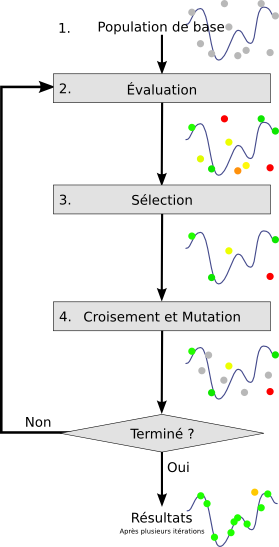
\includegraphics[width=.4\textwidth]{images/AG.png}
		\caption{Exemple d'algorithme génétique (source : wikipedia)}\label{fig:AG}
	\end{figure}


Si il est tout à fait logique que les algorithmes génétiques répondent parfaitement à la définition de l'évolution par sélection naturelle puisque ils ont été créés pour le faire, il est néanmoins intéressant de remarquer à quel point les roboticiens n'ont pas eu trop à les distordre pour s'en servir.
En effet, là où les informaticiens en algorithmique évolutionnaire classique ont souvent du ruser, détourner et ajouter de nombreux mécanismes \emph{ad-hoc} et sans équivalent biologique aux principes de base pour répondre aux problèmes qui leur étaient posés, les roboticiens n'ont bien souvent eux qu'à reprendre les premières formulations des algorithmes génétiques, superposables quasi parfaitement avec la définition de Lewotin, pour obtenir de très bon résultats (pour une revue assez complète, voir \citet{nolfi00evolrobobiolintetechselfmach}, pour une revue plus récente : \citet{floreano10evolutionadaptivebehaviourrobotsbymeansdarwinianselection}).

Tout comme en Informatique Évolutionnanrei les nuances et les ``écoles'' sont nombreuses. Il existent de nombreuses ``approches'' possibles.%citer la famille sisi
\subsection{Niveau de sélection et composition des groupes \citep{waibel09geneticteamcompositionlevelselectionevolutioncooperation}}\label{sec:nscg}

Dans cette étude les auteurs veulent tester différentes méthodes de sélection sur différents groupes de robots. Ils le font dans l'optique de quantifier l'efficacité de différentes approches pour programmer automatiquement des robots. Nous allons essayer de montrer que ces résultats peuvent être analysés et interprétés différemment si on les éclaire à lumière des débats discutés précédemment (cf \ref{sec:lvl}).

Pour réaliser leur étude les auteurs proposent trois tâches dans lesquelles différents niveaux d'altruisme (1. pas d'altruisme,2. coopération,3.  altruisme) sont nécessaires.
Dans les trois tâches des groupes de robots doivent déplacer des jetons vers une zone particulière (peinte en blanc) d'une arène. Dans la tâche où aucune coopération n'est nécessaire, les robots doivent déplacer des petits jetons qu'un robot seul peut pousser. Chaque fois qu'un robot ramène un de ces jetons, sa fitness est augmentée de un. Dans la tâche où la coopération\footnote{Nous considérons l'altruisme comme un acte de coopération qui n'offre aucun avantage sélectif à l'individu qui coopère mais en donne à l'autre. Lors d'un acte de coopération ``classique'' les deux protagonistes gagnent à coopérer.} est requise, il faut déplacer des gros jetons qui ne sont déplaçables que part au moins deux robots. Lorsqu'un gros jeton est ramené, la fitness de \emph{tous} les robots de l'expérience est augmentée de un, que les robots aient ou non participé au déplacement du jeton. Dans la dernière tâche les deux types de jetons sont présents, les mêmes systèmes de distribution des points de fitness que les tâches précédentes sont repris.

Les comportements seront contrôlés par un réseau de neurones artificiels assez simple\footnote{Un perceptron mutli couches.} reliant des capteurs infrarouges qui permettent au robot d'éviter les obstacles, une caméra qui permet différencier les jetons et de voir la zone blanche (un mur), et les moteurs qui contrôlent les roues pour déplacer le robot.
Les auteurs vont ensuite, par évolution artificielle, faire évoluer les paramètres de ces contrôleurs pour que les robots soient capables de résoudre les tâches imposées, en étudiant deux aspects particuliers de leur stratégie de sélection : le niveau auquel la sélection s'effectue et la composition des groupes sur lesquels elle opère. 

Par niveau de sélection les auteurs entendent la chose suivante : dans un algorithme d'évolution artificielle (cf section \ref{sec:ae}) des comportements sont générés aléatoirement, puis testés et évalués sur des robots dans l'environnement (réel ou simulé). \`A l'issue de ces tests le robot obtient une valeur de \emph{fitness} qui servira pour sélectionner les meilleurs individus. Mais le problème est de savoir si, lors d'une tâche dans laquelle une coopération est nécessaire, il ne vaut pas mieux sélectionner une populations au complet ayant bien résolu la tâche plutôt qu'un individu seul ayant une fitness élevé, au risque de ne sélectionner que des individus égoïstes. 

Pour comprendre ce que les auteurs entendent par composition des groupes il faut essayer de mieux comprendre l'expérience. Pour faire évoluer les comportements des robots les chercheurs doivent générer un certain nombre de groupes et tester l'efficacité de ces groupes à résoudre la tâches. Il faut ensuite constituer les générations suivantes en générant de nouveaux groupes en fonction des résultats des groupes initiaux. Mais comment doivent être constitués les groupes initiaux et les groupes des générations suivantes ? Avec des individus similaires ou différents ? Les générations suivantes doivent-elles être constituées de groupes homogènes composés de descendants des meilleurs individus des générations précédentes, ou bien d'un mix des individus des meilleurs groupes? Voilà la question derrière ``composition des groupes''. Que se passe-t-il si nous avons des groupes uniformes ``génétiquement'', dont les individus sont les ``clones'' de la même ``souche'' (ce qui est par exemple le cas pour les cellules d'un organisme pluricellulaire ou d'une colonie de fourmis) ou si les populations des générations N+1 sont composé de mixtes aléatoires des descendants des meilleurs individus de la génération N.

En couplant ces questions à celles sur les niveaux de sélection les auteurs veulent voir si certains types de sélection (groupe vs individu) favorisent l'évolution de certaines caractéristiques (altruisme) suivant les groupes sur lesquels la sélection opère (groupes homogènes vs hétérogènes). On peut imaginer par exemple que, dans le cas de la tâche où l'évolution de l'altruisme est nécessaire, si les meilleurs individus sont sélectionnés dans des groupes hétérogènes, il sera possible de sélectionner des individus égoïstes d'autant plus si ils ont été testés dans des groupes avec beaucoup d'altruistes. Les groupes des générations suivantes seront donc peu performants à la tâche puisque composés uniquement d'égoïstes et donc incapables de pousser les gros jetons qui maximiseraient leur fitness. Alors que si la sélection s'opère sur les groupes, les groupes des générations suivantes, composé de mix d'individus choisis aléatoirement dans les meilleurs groupes d'individus, auront des chances d'être composés d'altruistes et donc de réussir la tâche.

Bien qu'ici posées dans un cadre d'optimisation et d'ingénieurie, ces questions sont exactement celles que biologistes et philosophes se posent. L'idée est donc de transférer les résultats des ces expériences à la biologie. Mais en le faisant un certain nombre de précautions doivent être prises et il faut garder à l'esprit que ces expériences se font dans un cadre et selon un protocoles très particulier, qu'il convient de considérer avec attention. Il faut donc bien vérifier que le système biologique auquel on veut appliquer l'analogie corresponde au protocole expérimental si on veut pouvoir étendre les résultats de l'expérience en robotique à un système biologique particulier.  


Nous ne rentrerons pas dans le détails des résultats de l'expérience et n'en présenterons que l'essentiel. Dans tout les cas les algorithmes d'évolution artificielle sont capable de faire évoluer les comportements adéquats pour résoudre les t\^aches demandées, ce qui irait dans le sens de certains pluralistes qui considèrent que la sélection de groupes peut exister conjointement à la sélection individuel, les deux n'étant que le reflet d'un même phénomène observé différemment. 
Néanmoins des différences significatives dans la \emph{vitesse de convergence}\footnote{Rapidité de l'algorithme à trouver des comportements adéquats} ou dans la qualité des solutions obtenues sont observables. En règle générale les tâches ne nécessitant pas de coopération sont mieux réussies par des groupes hétérogènes, tandis que la sélection (individuelle ou de groupe) au sein de groupes homogènes est plus efficace pour les tâches où la coopération est nécessaire. Les auteurs analysent les raisons de ces différences pour essayer d'en comprendre les causes, et c'est là que le biologiste doit être vigiliant. Car avant d'étendre ces résultats à un système biologique le chercheur doit faire très attention à ce que le protocole expérimental appliqué par les roboticiens corresponde à son système biologique. La façon dont la ``sélection de groupes'' a été implémentée peut-elle correspondre à la façon dont l'objet biologique est sélectionné? le mode de propagation, les tailles de populations, etc.. toutes ces variables doivent être étudiées et comparées si l'on veut situer l'étendu et la valeur des informations que le modèle peut fournir au biologiste. D'autant plus que ces protocoles n'ont pas été pensés initialement pour répondre à des problèmes biologiques, mais d'ingénieurie.




\section{citation}
\begin{quote}
	It is, therefore, of the highest importance to gain a clear insight into the means of modification and coadaptation. At the commencement of my observations it seemed to me probable that a careful study of domesticated animals and of cultivated plants would offer the best chance of making out this obscure problem. Nor have I been disappointed; in this and in all other perplexing cases I have invariably found that our knowledge, imperfect though it be, of variation under domestication, afforded the best and safest clue. I may venture to express my conviction of the high value of such studies, although they have been very commonly neglected by naturalists.\footnote{\citet[Introduction p. 27 ]{darwin1859originspeciesbymeansnaturalselectionorpreservationfavouredracesstrugglelife}}
\end{quote}

\footnote{Nous verrons dans la partie \ref{ch:RE} que la RE tombe effectivement dans cette catégorie et est perçue comme ça par ces acteurs. Néanmoins son rapprochement avec la Vie Artificielle n'est pas donné \emph{a priori} et relève plus d'une volonté de la communauté : la RE aurait très bien pu ce développer en modèle d'ingénierie loin des considérations de la vie artificielle.}


\section{Geoarge Gaylord Simpson}
la 



For instance, models can be used as epistemic tools to understand how natural systems work, to explain life and living phenomena, making explicit and tractable the underlying universal principles of biological organization by exploring properties of complex systems and simulating some specific natural behaviour.    The emergent order that natural systems show can also be seen as the unfolding of a functional evolutionary design that turns out to be attractive for engineering goals. In fact, evolution is an extremely accurate blind engineer that can teach us weird and new ways of achieving solutions for a wide range of problems. Both the organization of individual living systems and their collective behaviour (e.g. colonies) also give rise to intriguing designs and functional behaviours. Nature is not constrained by any theoretical assumption, design principles or industrial tradition, and thus becomes an attractive pool, in which original and sophisticated, simple but powerful engineering techniques can be found. Finally, under aesthetic purposes biologically inspired artefacts can also be used to produce pleasant and original visual or musical patterns.
\cite{barandiaran06alifemodelsasepistemicartefacts}
